\section{Methodik}
\subsection{Softwarearchitektur}
\subsection{Kennzeichenerkennung}
Die Kennzeichenerkennung ist ein Verfahren der Bildverarbeitung, das zur Erkennung und Interpretation von Fahrzeugkennzeichen auf Bildern oder Videoaufnahmen eingesetzt wird. Sie findet Anwendung in zahlreichen Bereichen wie der Verkehrsüberwachung, Mauterfassung, Parkraumbewirtschaftung oder Zufahrtskontrolle.\\\\
Das System basiert im Wesentlichen auf drei zentralen Prozessschritten: der Bilderfassung, der Lokalisation des Kennzeichens im Bild sowie der Texterkennung. Zunächst wird ein Bild eines Fahrzeugs aufgenommen, durch eine Kamera. Im nächsten Schritt wird das Kennzeichen im Bild identifiziert dies geschieht mithilfe moderner Objekterkennungsalgorithmen wie YOLO oder klassischer Verfahren der Konturenerkennung. Nachdem der relevante Bildausschnitt extrahiert wurde, folgt die optische Zeichenerkennung, bei der die alphanumerischen Zeichen des Kennzeichens ausgelesen und digital erfasst werden.\\\\
Die Genauigkeit der Kennzeichenerkennung hängt stark von der Qualität der Vorverarbeitung ab, bei der Methoden wie Graustufenumwandlung, Rauschfilterung, Binarisierung und Kantenanalyse eingesetzt werden, um ein möglichst klares Bild für die Texterkennung zu erzeugen. Moderne Systeme kombinieren dabei klassische Bildverarbeitung mit maschinellem Lernen, um auch bei schwierigen Lichtverhältnissen, verzerrten Perspektiven oder verunreinigten Kennzeichen verlässliche Ergebnisse zu erzielen.

\subsubsection{Systemarchitektur und Funktionsweise}
Das implementierte System zur Kennzeichenerkennung basiert auf einer Kombination aus Hardware- und Softwarekomponenten. Für die grundlegende Funktionsfähigkeit werden folgende Hardware-Voraussetzungen benötigt: ein Raspberry Pi oder ein funktionsfähiger Computer, eine handelsübliche oder integrierte Webcam, eine SD-Karte mit dem entsprechenden Betriebssystem-Image für den Raspberry Pi sowie eine Tastatur, Maus und ein HDMI-Kabel zur Verbindung mit einem Monitor. Alternativ können Tastatur, Maus und HDMI-Kabel entfallen, wenn der Raspberry Pi über den RealVNC Viewer ferngesteuert und eingerichtet wird.\singlespacing 
Auf der Softwareseite kommen verschiedene Technologien zum Einsatz. Zur Objekterkennung wird das Modell YOLOv5 verwendet, während OpenCV zur Bildverarbeitung und Tesseract OCR für die Texterkennung eingesetzt werden. \singlespacing
Der Ablauf der Kennzeichenerkennung erfolgt in drei Schritten: \\
1. Bilderfassung: Die Kamera nimmt acht Bilder auf, die lokal auf dem Gerät gespeichert werden.\\
2. Erkennung: Die gespeicherten Bilder werden mithilfe von YOLOv5 analysiert. Die erkannten Kennzeichenbereiche (Bounding Boxes) werden markiert und die Bilder erneut gespeichert. \\
3. Texterkennung: Im letzten Schritt erfolgt die optische Zeichenerkennung (OCR) mit Tesseract. Dabei werden die Buchstaben extrahiert, separat gespeichert und das erkannte Kennzeichen im Konsolenfenster ausgegeben. \\

Das System wurde speziell am Beispiel für den Einsatz an europäischen Mautstationen konzipiert und optimiert.

\subsubsection{Training und Optimierung des Modells}
Für die Erkennung der Kennzeichenbereiche wurde bewusst das Modell YOLOv5 eingesetzt. Dieses Modell bietet eine ausgewogene Kombination aus Genauigkeit und Effizienz und eignet sich besonders gut für ressourcenbeschränkte Umgebungen wie den Raspberry Pi. Zwar existieren mittlerweile neuere und theoretisch leistungsfähigere Modellversionen, doch diese bringen meist deutlich höhere Anforderungen an Rechenleistung und Speicher mit sich, was eine stabile Ausführung auf einem Mikrocomputer wie dem Raspberry Pi erschwert oder sogar unmöglich macht. Gerade im Hinblick auf die beschränkten Hardwarekapazitäten des Raspberry Pi ist YOLOv5 insbesondere in den Varianten „nano“ oder „small“ eine sinnvolle Wahl. Diese Varianten sind speziell darauf ausgelegt, auch auf schwächerer Hardware zuverlässig zu funktionieren und dabei dennoch eine ausreichend hohe Erkennungsgenauigkeit zu gewährleisten. In der Praxis zeigt sich, dass mit YOLOv5 eine robuste Objekterkennung in nahezu Echtzeit möglich ist, ohne den Systembetrieb zu beeinträchtigen.\\

Zur Detektion von KFZ-Kennzeichen im Bildmaterial kommt in unserem Projekt ein speziell trainiertes YOLOv5-Modell zum Einsatz. YOLO  ist eine auf Echtzeit ausgelegte Objekterkennungsarchitektur, die es ermöglicht, Objekte wie Nummernschilder direkt in Bildern zu lokalisieren und zu klassifizieren. Wir haben uns dabei für die besonders kompakte Variante YOLOv5n (nano) entschieden, da diese für ressourcenschwache Systeme wie den Raspberry Pi 4 optimiert ist und eine hohe Inferenzgeschwindigkeit bei geringer Modellgröße bietet.

\paragraph{Datengrundlage}

Als Trainingsgrundlage diente ein öffentlich zugänglicher Datensatz aus Roboflow Universe mit rund 3.000 annotierten Bilder von KFZ-Kennzeichen\footnote{\url{https://universe.roboflow.com/roboflow-universe-projects/license-plate-recognition-rxg4e}}. Der Datensatz enthält bereits diverse Perspektiven, Lichtverhältnisse und Rotationen, was zur Robustheit des Modells beiträgt.\\

Zusätzlich wurden während des Trainings verschiedene Datenaugmentierungen vorgenommen, um die Generalisierungsfähigkeit weiter zu verbessern. Hierzu zählten unter anderem:

\begin{itemize}
    \item Auto-Orientierung zur Korrektur der Bildausrichtung
    \item Resize auf ein einheitliches Format von 640x640 Pixel
    \item Rauschüberlagerung (bis zu 1{,}6\% der Pixel)
    \item Unschärfeeffekte (bis zu 1{,}6\% Pixel Blur)
  \end{itemize}

Diese Maßnahmen wurden mit Roboflow automatisiert vorgenommen. Das Modell wurde anschließend in Google Colab auf einer GPU-Instanz trainiert. Die Trainingsdauer betrug etwa 1,5 bis 2 Stunden. Als Hyperparameter wurden 50 Epochen mit einer Batch-Größe von 10 verwendet. Die restlichen Parameter (zum Beispiel Lernrate) blieben auf den Standardwerten des YOLOv5-Frameworks.

\paragraph{Trainingsergebnisse und Validierung}{}

Zur Bewertung des Trainingsverlaufs wurden typische Metriken von YOLOv5 analysiert. Abbildung~\ref{fig:training} zeigt die Entwicklung der Kennzahlen über den Verlauf von 50 Trainings-Epochen.\\

\begin{figure}[h]
    \centering
    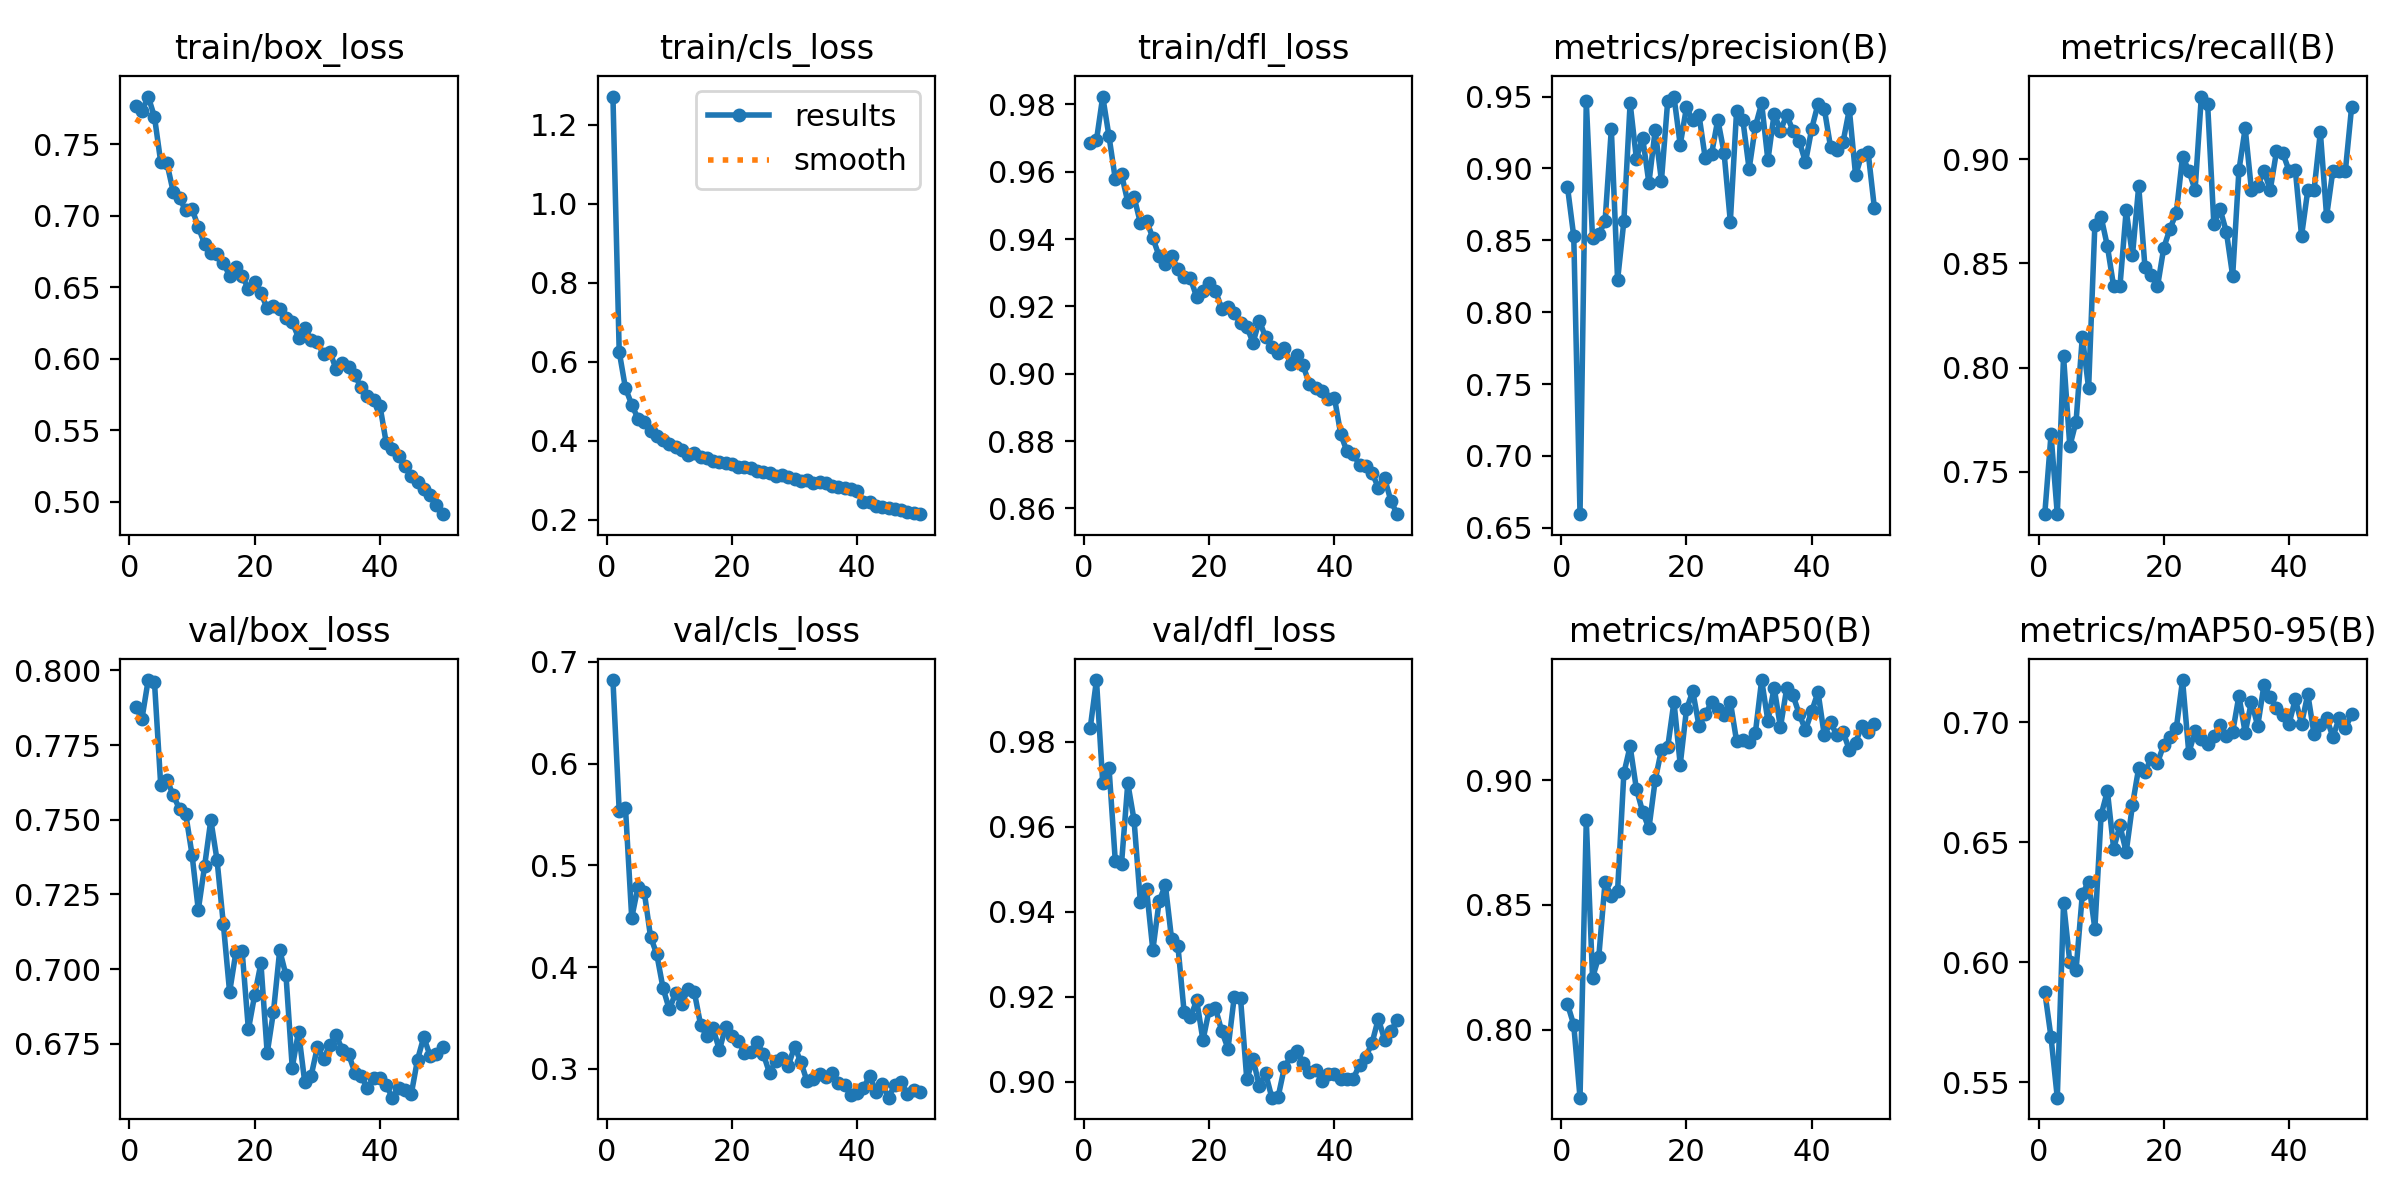
\includegraphics[width=0.55\textwidth]{data/training_results.png}
    \caption{Trainingsergebnisse des YOLOv5-Modells.}
    \label{fig:training}
\end{figure}

Zu erkennen ist, dass sowohl die Trainings- als auch Validierungsverluste (box\_loss, cls\_loss, dfl\_loss) im Verlauf kontinuierlich abnehmen, was auf ein stabiles und erfolgreiches Training hindeutet. Besonders der Klassifikationsverlust (cls\_loss) zeigt eine schnelle Konvergenz in den ersten zehn Epochen. Die Präzision und der Recall pendeln sich im oberen Bereich ein – teils mit leichten Schwankungen, die jedoch durch das kleine Modell und die geringe Batch-Größe erklärbar sind.\singlespacing

Besonders relevant ist der mean Average Precision (mAP) – ein Maß für die Genauigkeit bei verschiedenen IoU-Schwellenwerten. Der Wert mAP@0.5 steigt im Verlauf des Trainings auf über 0,9, während mAP@0.5:0.95 einen stabilen Endwert um 0,70 erreicht. Dies spricht für eine hohe Detektionsqualität, auch bei komplexeren Szenarien.
\paragraph{Konfidenz und Modellanwendung}
Die Ausgabe eines YOLO-Modells enthält neben den erkannten Objektpositionen auch sogenannte Konfidenzwerte, also Wahrscheinlichkeiten, mit denen das Modell ein Objekt als erkannt einstuft. In unserem Projekt wurde ein Konfidenzschwellenwert definiert, um falsch-positive Erkennungen zu reduzieren. Nur Detektionen mit einer Konfidenz über diesem Schwellenwert wurden weiterverarbeitet.\singlespacing

Das trainierte YOLOv5-Modell im .pt-Format wurde zur Performanzoptimierung in das NCNN-Format konvertiert. NCNN ist ein hochoptimiertes Inferenz-Framework speziell für mobile und eingebettete Systeme. Dadurch konnte das Modell auf dem Raspberry Pi 4 mit hoher Effizienz ausgeführt werden. Die Anwendung läuft in einem Skript, das serienweise acht Bilder aufnimmt und analysiert – was nahezu Echtzeitverarbeitung ermöglicht.

\paragraph{Einfluss der Trainingsdaten und Verbesserungsmöglichkeiten}
Die Qualität und Diversität der Trainingsdaten hat direkten Einfluss auf die Erkennungsleistung. In unserem Fall war der Datensatz breit gefächert, jedoch auf Kennzeichen fokussiert. Mögliche Optimierungen für die Zukunft wären:

\begin{itemize}
    \item Erweiterung des Datensatzes um reale eigene Aufnahmen
    \item Feinjustierung der Augmentierungstechniken
    \item Transfer Learning mit größeren Basismodellen
    \item Active Learning durch gezieltes Nachtraining mit fehlerhaften Beispielen
  \end{itemize}

  Dadurch könnte die Robustheit des Modells gezielt für Spezialfälle wie Nachtaufnahmen, verschmutzte Kennzeichen oder ungewöhnliche Kamerawinkel verbessert werden.


\subsubsection{Image Preprocessing}

Die Bildvorverarbeitung dient der Verbesserung der visuellen Eigenschaften der Bildausschnitte, in denen die Nummernschilder enthalten sind. Ziel ist es, die Zeichenstrukturen klar hervorzuheben, Bildrauschen zu minimieren und die Voraussetzungen für eine spätere Weiterverarbeitung, beispielsweise durch Texterkennung, zu schaffen.\singlespacing

Der erste Schritt der Pipeline besteht in der Umwandlung des Originalbildes in ein Graustufenbild. Dieses wird anschließend um den Faktor 3 vergrößert, um relevante Details, insbesondere feine Strukturen von Zeichen, deutlicher hervorzuheben. Im Anschluss erfolgt eine Glättung mittels eines Gaußschen Weichzeichners mit einer Kernelgröße von 3$\times$3, um Bildrauschen zu unterdrücken.

Darauf folgt ein binäres Thresholding mit inversierter Darstellung (\texttt{cv2.THRESH\_BINARY\_INV}). Durch diese Umkehrung erscheinen potenzielle Zeichenbereiche weiß auf schwarzem Hintergrund, was die spätere Konturerkennung erleichtert.\singlespacing

Um benachbarte Strukturen zu verbinden und kleinere Lücken in Zeichenformen zu schließen, wird im nächsten Schritt eine morphologische Dilation durchgeführt. Hierbei wird ein rechteckiges Strukturierungselement der Größe 3$\times$3 verwendet.\singlespacing

Die vorbereiteten Bilder werden im Anschluss zur Konturerkennung verwendet, wobei die Konturen in der Regel einzelnen Zeichen oder Zeichenkomponenten entsprechen. In späteren Verarbeitungsschritten können diese Bereiche gezielt extrahiert und analysiert werden.\singlespacing

Durch diese Kette an Vorverarbeitungsschritten wird sichergestellt, dass relevante Bildinformationen betont und störende Einflüsse reduziert werden, um die Qualität der anschließenden Bildanalyse zu maximieren.


\subsubsection{Optical Character Recognition}

Nach Abschluss der Bildvorverarbeitung, bei der die Kennzeichenbilder in eine geeignete Form gebracht wurden, erfolgt die Erkennung der enthaltenen alphanumerischen Zeichen mittels Optical Character Recognition (OCR). Zu Beginn des Projekts wurden dazu verschiedene OCR-Engines untersucht, darunter auch EasyOCR. Diese Deep-Learning-basierte Bibliothek liefert in vielen Anwendungsfällen gute Ergebnisse, zeigte jedoch im praktischen Einsatz auf ressourcenschwacher Hardware wie dem Raspberry Pi 4 deutliche Einschränkungen. Der hohe Speicherbedarf und die langen Inferenzzeiten verhinderten eine Echtzeitverarbeitung.\singlespacing

Im Vergleich dazu bot Tesseract eine deutlich geringere Systemlast bei gleichzeitig stabiler Erkennungsleistung. Besonders in unserem Anwendungsfall – kontrastreiche, segmentierte Kennzeichenbilder – erwies sich Tesseract als ausreichend genau. Durch gezielte Konfigurationsmöglichkeiten, wie die Beschränkung auf bestimmte Zeichensätze und Layout-Modi, ließ sich die Leistung zusätzlich optimieren. Aus diesen Gründen fiel die Entscheidung auf die Kombination aus Tesseract und der Python-Bibliothek \texttt{pytesseract}.\singlespacing

Im nächsten Schritt der Pipeline erfolgt eine Konturanalyse auf dem vorbereiteten binären Bild. Die erkannten Konturen werden nach verschiedenen geometrischen Kriterien gefiltert, um nur relevante Regionen weiterzuverarbeiten – etwa anhand von Größe, Seitenverhältnis und Position. Für jede verbleibende Kontur wird ein leicht vergrößerter Bildausschnitt (Region of Interest) definiert. Dieser wird an die OCR-Engine übergeben.\singlespacing

Die Texterkennung wird über die Funktion \texttt{image\_to\_data} durchgeführt. Dabei wird der zu analysierende Zeichensatz auf Großbuchstaben und Ziffern eingeschränkt (\texttt{tessedit\_char\_whitelist}) und mit dem Seitenlayout-Modus \texttt{--psm 8} gearbeitet, der für einzelne Zeichen geeignet ist. Das Ergebnis umfasst neben dem erkannten Text auch Positionsdaten und Konfidenzwerte.\singlespacing

Abschließend werden die erkannten Zeichenbereiche im Graustufenbild visuell hervorgehoben und als Bilddateien gespeichert, um die Ergebnisse nachvollziehbar und prüfbar zu machen.

\subsubsection{Herausforderungen bei realen Bedingungen}
Im Rahmen der Entwicklung unseres Kennzeichenerkennungssystems, das auf eine Mautstationssituation ausgelegt ist, traten verschiedene Herausforderungen auf, die unter realen Bedingungen von besonderer Bedeutung sind. \singlespacing

Eine der ersten Schwierigkeiten bestand in der Vielfalt von Kfz-Kennzeichen weltweit. 
Während die Objekterkennung des Kennzeichens selbst (die Lokalisierung auf dem Bild) zuverlässig funktionierte, erwies sich das anschließende Auslesen der Schriftzeichen als problematisch. 
 Dies lag an den unterschiedlichen Formaten, Schriftarten und Normen, die international variieren. 
 Nach eingehender Analyse kamen wir zu dem Entschluss, dass die Entwicklung eines universellen Kennzeichenerkenners, der alle internationalen Standards abdeckt, den Rahmen unseres Projektes deutlich überschreiten würde. 
 Stattdessen entschieden wir uns, eine optimierte Lösung speziell für deutsche Kfz-Kennzeichen zu entwickeln, um innerhalb der gegebenen Projektgrenzen eine funktional stabile Erkennung zu gewährleisten.\singlespacing
 Eine weitere Herausforderung stellte die Anpassung des Systems an verschiedene Licht- und Schattenbedingungen dar. 
 Schon bei kleinen aber vor allem bei stark wechselnden Beleuchtungsverhältnissen war die Festlegung geeigneter Thresholds bei der Bildverarbeitung für eine universale Lösung herausfordernd. 
 Auch hier zeigte sich, dass eine umfassende allgemeine Lösung, die alle möglichen Umgebungsbedingungen robust abdeckt, einen erheblichen zusätzlichen Entwicklungsaufwand erfordern würde. \singlespacing
 Zudem stießen wir auf technische Grenzen hinsichtlich der Leistungsfähigkeit des eingesetzten Raspberry Pi.
Insbesondere die Schriftzeichenerkennung stellte hohe Anforderungen an die Prozessorleistung, was die Echtzeitfähigkeit des Systems deutlich beeinträchtigte.
Es wurde schnell klar, dass der Raspberry Pi vor allem für den Einsatz unter kontrollierten Laborbedingungen geeignet ist, während für Anwendungen unter realen Bedingungen leistungsstärkere Hardware empfohlen wird.
Die Herausforderung lag hier insbesondere darin, eine akzeptable Balance zwischen Hardwareanforderungen und Systemleistung herzustellen.\singlespacing

Vor diesem Hintergrund entschieden wir uns bewusst für die Verwendung der YOLOv5-Architektur, da diese im Vergleich zu neueren Modellen wie YOLOv8 eine deutlich geringere Rechenlast aufweist und damit besser auf ressourcenbeschränkter Hardware wie dem Raspberry Pi lauffähig ist.
Die Wahl eines leichteren Modells ermöglichte es, die grundlegenden Funktionen der Gesichts- und Schrifterkennung trotz der beschränkten Systemressourcen zuverlässig zu demonstrieren. 
\subsubsection{Optimierung für wechselnde Lichtverhältnisse und Kameraperspektiven}

Zur Verbesserung der Erkennungsstabilität unter realen Bedingungen wird besonderes Augenmerk auf die Bildverarbeitung gelegt. Ein vielversprechender Ansatz besteht in der Nutzung mehrstufiger Preprocessing-Pipelines. Hierbei wird dasselbe Eingangsbild mehreren parallel ausgeführten Vorverarbeitungsschritten unterzogen, die jeweils auf typische Problemquellen wie Überbelichtung, Schatten oder Kontrastarmut optimiert sind. Die resultierenden Varianten werden anschließend bewertet, um die am besten geeignete für die Texterkennung auszuwählen.\singlespacing

Darüber hinaus kann perspektivische Verzerrung durch geometrische Transformationen, etwa mithilfe von Homographie-Matrizen, reduziert werden. Diese Maßnahme ist besonders bei schräg aufgenommenen Kennzeichenbildern sinnvoll, wie sie bei ungünstiger Kameraposition oder ungleichmäßiger Fahrzeugausrichtung entstehen.\singlespacing

Als mögliche Erweiterung wäre ein Postprocessing-Konzept denkbar, bei dem erkannte Zeichenfolgen hinsichtlich ihrer strukturellen Korrektheit überprüft werden. In professionellen Systemen wird dies häufig durch Plausibilitätsprüfungen oder den Vergleich mehrerer Verarbeitungsergebnisse realisiert. Dabei kommen Algorithmen zum Einsatz, die verschiedene OCR-Ergebnisse anhand formaler Merkmale, Zeichensatzvalidität und Konfidenzwerten bewerten, um das wahrscheinlich korrekteste Resultat zu ermitteln. Denkbar wäre zudem der Einsatz eines speziell trainierten KI-Modells, das ausschließlich auf die Erkennung von Schriftarten in KFZ-Kennzeichen ausgelegt ist. Ein solches Modell könnte Unsicherheiten der allgemeinen OCR durch domänenspezifisches Wissen kompensieren und die Gesamterkennungsrate unter realen Bedingungen deutlich verbessern.

\subsubsection{Evaluation und Genauigkeitsanalyse}


\subsection{Gesichtserkennung}
\subsubsection{Testaufbau}
Das implementierte System realisiert eine Echtzeit-Gesichtserkennung mittels einer handelsüblichen Webcam (640$\times$480 Pixel) und verwendet das Modell \texttt{YOLOv8n-face} zur Detektion von Gesichtern. Die Identifikation erfolgt durch Kombination der YOLO-basierten Gesichtserkennung mit dem \texttt{face\_recognition}-Framework, das HOG-basierte Merkmalsextraktion nutzt. Bekannte Gesichter werden im lokalen Verzeichnis gespeichert und können über eine grafische Benutzeroberfläche dynamisch erweitert werden. Das System ist für Zutrittskontrollszenarien konzipiert und erlaubt das Anlernen neuer Gesichter im laufenden Betrieb.

\subsubsection{YOLO}
\paragraph{Vergleich der YOLO-Modelle}
\begin{table}[h]
    \centering
    \begin{tabular}{|l|c|c|c|c|l|}
    \hline
    \textbf{Modell} & \textbf{mAP (face)} & \textbf{Inferenzzeit (ms)} & \textbf{Parameter} & \textbf{FLOPs} & \textbf{Besonderheiten} \\
    \hline
    YOLOv8n-face   & 39{,}2\%   & 80{,}4   & 3{,}2 Mio. & 8{,}7 Mrd. & Auf Gesichtserkennung spezialisiert \\
    YOLOv8n        & 37{,}3\%   & 80{,}4   & 3{,}2 Mio. & 8{,}7 Mrd. & Generelles Objekterkennungsmodell   \\
    YOLOv11n-face* & 41{,}5\%*  & 56{,}1   & 2{,}6 Mio. & 6{,}5 Mrd. & Verbesserte Architektur, schneller  \\
    \hline
    \end{tabular}
    \caption{Vergleich der wichtigsten YOLO-Modelle für die Gesichtserkennung. *Werte für YOLOv11n-face sind geschätzt, basierend auf aktuellen Trends in der YOLO-Architektur.}
    \end{table}
    
    Das auf Gesichter spezialisierte Modell YOLOv8n-face erzielt eine höhere Genauigkeit als das generische YOLOv8n. Das neuere YOLOv11n-face bietet voraussichtlich noch bessere Erkennungsraten und eine deutlich schnellere Inferenz, erfordert jedoch ggf. Anpassungen und erneutes Training für die Kompatibilität mit dem aktuellen Code. Generische Modelle wie YOLOv8n erkennen mehr Objekttypen, sind aber für die reine Gesichtserkennung weniger effizient.

\paragraph{Metriken}
Für die Bewertung der Gesichtserkennung sind folgende Metriken relevant:
\begin{itemize}
    \item \textbf{Precision (Genauigkeit):} Anteil der korrekt erkannten Gesichter an allen als erkannt gemeldeten Gesichtern.
    \item \textbf{Recall (Sensitivität):} Anteil der korrekt erkannten Gesichter an allen tatsächlich vorhandenen Gesichtern.
    \item \textbf{F1-Score:} Harmonisches Mittel aus Precision und Recall.
    \item \textbf{Inferenzgeschwindigkeit:} Anzahl der Bilder pro Sekunde (FPS) bzw. durchschnittliche Latenz pro Bild.
\end{itemize}

\paragraph{Python-Code zur Visualisierung}
%Python Diagramm

Zur Auswertung können folgende Attribute der \texttt{ultralytics}-Bibliothek genutzt werden:
\begin{itemize}
    \item \texttt{results.box.map50} für mAP@0.5 (mean Average Precision)
    \item \texttt{results.speed} für Inferenzzeit (ms pro Bild)
\end{itemize}

\paragraph{Anwendungsbeispiel: Zutrittskontrollen}
Das System ermöglicht eine zuverlässige Gesichtserkennung für Zutrittskontrollsysteme mit folgenden Eigenschaften:
\begin{itemize}
    \item Echtzeit-Erkennung mit einer Latenz von unter 250\,ms pro Bild.
    \item Visuelles Feedback durch Markierung und Beschriftung erkannter Gesichter im Videostream.
    \item Dynamisches Anlernen neuer Nutzer durch interaktive Eingabe.
    \item Speicherung der Gesichtsdaten in einem lokalen Verzeichnis; Erweiterung durch SQLite möglich.
    \item Erweiterbar für Multi-Faktor-Authentifizierung (z.\,B. RFID + Gesicht).
\end{itemize}

\textbf{Ergebnisse:} In kontrollierter Umgebung erreicht das System eine Erkennungsrate von ca.~93\,\%. Bei schwierigen Lichtverhältnissen sinkt die Rate auf etwa 78\,\%. Für produktive Anwendungen empfiehlt sich die Ergänzung durch IR-Kameras und Liveness Detection.

\begin{quote}
Das vorgestellte System kombiniert die Geschwindigkeit und Präzision moderner YOLO-Modelle mit der Flexibilität des Face-Recognition-Frameworks und ist damit für den Einsatz in sicherheitskritischen Zutrittskontrollen geeignet.
\end{quote}

\subsubsection{MediaPipe}
\paragraph{Gesichtspunkterkennung: Code} 

Für die Gesichtspunkterkennung nutzen wir das FaceMesh Modell von Mediapipe, das 468 3D-Gesichtspunkte in Echtzeit erfasst. Diese dreidimensionalen Koordinaten ermöglichen vielfältige Anwendungen in Gesichtserkennung, Emotionsanalyse und Augmented Reality.

(?) Der vollständige Code, der die hier beschriebene Gesichtspunkt-Erkennung mit MediaPipe implementiert, ist im Anhang und/oder auf GitHub verfügbar.
Der ganze Code ist in Python geschrieben.

Zunächst müssen wir notwendigen die Bibliotheken importieren. Diese sind in unserem Fall die OpenCV und MediaPipe-Bibliotheken.
Danach initialisieren wir die MediaPipe-Instanz. Dies geschieht mit dem folgenden Code:
\begin{lstlisting}
    # MediaPipe FaceMesh Setup
    mp_face_mesh = mp.solutions.face_mesh
    face_mesh = mp_face_mesh.FaceMesh(static_image_mode=False, max_num_faces=5, min_detection_confidence=0.8)
\end{lstlisting}

\textbf{Parameter-Erläuterung:}
\begin{itemize}
    \item \texttt{static\_image\_mode=False}: Entscheidend für die Verarbeitung von Videostreams und Live-Kameraaufnahmen, signalisiert dem Modell eine Bildsequenz.
    \item \texttt{max\_num\_faces=5}: Begrenzt die Erkennung auf maximal 5 Gesichter gleichzeitig.
    \item \texttt{min\_detection\_confidence=0.8}: Setzt die Erkennungsschwelle auf 80\% für präzise Resultate bei guter Balance zwischen Genauigkeit und Robustheit.
\end{itemize}

Um die erkannten Gesichtspunkte und deren Verbindungen visuell darzustellen, initialisieren wir die Zeichenwerkzeuge von MediaPipe. \texttt{drawing\_spec} definiert das Aussehen der Punkte und Linien (z.B. Farbe, Dicke).

Im nächsten Schritt wird die Webcam geöffnet, um Videobilder aufzunehmen. Alternativ könnte man hier auch den Pfad zu einer Bild- oder Videodatei angeben. 

Die Hauptschleife des Programms läuft, solange die Kamera aktiv ist. In jeder Iteration der Schleife wird ein neues Bild von der Webcam erfasst und verarbeitet.

Ein wichtiger Schritt ist die Konvertierung des Farbraums des aufgenommenen Bildes von BGR (Blue, Green, Red), dem Standardformat von OpenCV, nach RGB (Red, Green, Blue), das von MediaPipe erwartet wird.
\begin{lstlisting}
    rgb_frame = cv2.cvtColor(frame, cv2.COLOR_BGR2RGB)
\end{lstlisting}
Diese Konvertierung ist notwendig, da unterschiedliche Bibliotheken und Modelle intern mit verschiedenen Farbreihenfolgen arbeiten. Die Verwendung der falschen Reihenfolge kann zu fehlerhaften Ergebnissen führen.

Nun verarbeitet MediaPipe das in RGB konvertierte Bild, um Gesichter zu erkennen und die entsprechenden Gesichtspunkte zu lokalisieren.

Sobald ein oder mehrere Gesichter im Bild erkannt wurden, zeichnen wir die 468 Gesichtspunkte und die Verbindungen zwischen ihnen auf das ursprüngliche Farbbild.
\begin{lstlisting}
    if results.multi_face_landmarks:
    for face_landmarks in results.multi_face_landmarks:
        # draw all landmarks
        mp_drawing.draw_landmarks(
            image=frame,
            landmark_list=face_landmarks,
            connections=mp_face_mesh.FACEMESH_TESSELATION,
            landmark_drawing_spec=drawing_spec,
            connection_drawing_spec=drawing_spec
        )
\end{lstlisting}
\textbf{Parameter-Erläuterung}:
\begin{itemize}
    \item \texttt{image=frame}: Das Originalbild (im BGR-Format) für die Visualisierung der Landmarken.
    \item \texttt{landmark\_list=face\_landmarks}: Die Liste der erkannten Gesichtspunkte für ein einzelnes Gesicht.
    \item \texttt{connections=mp\_face\_mesh.FACEMESH\_TESSELATION}: Die vordefinierten Verbindungen zwischen den Gesichtspunkten, die das FaceMesh Modell verwendet (z.B. um Augenbrauen, Lippen, Gesichtskonturen darzustellen).
    \item \texttt{landmark\_drawing\_spec=drawing\_spec}: Die zuvor definierten Zeichenstil-Spezifikationen für die einzelnen Punkte.
    \item \texttt{connection\_drawing\_spec=drawing\_spec}: Die zuvor definierten Zeichenstil-Spezifikationen für die Verbindungslinien.
\end{itemize}

Schließlich wird das mit den eingezeichneten Gesichtspunkten versehene Bild angezeigt. Die Schleife wird beendet und die Webcam freigegeben, sobald der Benutzer die ESC-Taste drückt oder das Programm manuell beendet.

Dieser Code bildet die Grundlage für unsere Gesichtswiedererkennung.

\paragraph{Gesichtswiedererkennung mit Gesichtspunkten: Code} 

Unser System zur Echtzeit-Gesichtserkennung nutzt MediaPipe FaceMesh, um Gesichter in Videostreams präzise zu erkennen.
Seine Funktionalität umfasst das Erlernen und Speichern neuer Gesichter, das Wiedererkennen bekannter Personen und die Fähigkeit zum kontinuierlichen Dazulernen, wodurch sich die Erkennungsleistung stetig verbessert.

Im Kern unseres Programms steht die Initialisierung, in der das MediaPipe FaceMesh-Modul eingerichtet und die Kamera gestartet wird, wie es in Abschnitt 4.3.3.1 beschrieben ist.
Zudem werden Speicherstrukturen für die Namen bekannter Gesichter und deren charakteristische Gesichtspunkte (Landmarks) vorbereitet.

Die eigentliche Gesichtserkennung erfolgt durch die Funktion \texttt{extract\_face\_landmarks}. Diese nutzt MediaPipe, um detaillierte Gesichtsmerkmale zu extrahieren, wobei ein besonderer Fokus auf 50 Schlüsselpunkte in den Bereichen Augen, Nase, Mund und Augenbrauen liegt.
Um eine konsistente Erkennung zu gewährleisten, werden die Koordinaten dieser Punkte normalisiert. Das heißt, dass sie relativ zur Gesichtsgröße und -position skaliert werden, um Verzerrungen durch unterschiedliche Perspektiven und Entfernungen zu minimieren.

Für den Gesichtsvergleich kommt die Methode \texttt{detect\_and\_recognize\_faces} zum Einsatz. Sie vergleicht neu erkannte Gesichtsmerkmale mit den gespeicherten Daten.
Dabei werden gewichtete Abstände zwischen den Punkten berechnet, wobei einzelnen Gesichtsregionen, insbesondere den Augen höhere Bedeutung zugewiesen wird, was die Genauigkeit der Erkennung erhöht.
\begin{lstlisting}
    # Continuous learning: Improved strategy for continuous learning
            # Only learn when recognition is relatively certain, but not perfect
            if is_known_face:
                # Low confidence: Try to learn
                if 0.6 < confidence < 0.95:
                    self.add_landmark_to_person(name, landmarks)
                # Very low confidence: Only learn occasionally (reduces false associations)
                elif 0.4 < confidence <= 0.6:
                    # Only learn in 30% of cases to reduce errors
                    if np.random.random() < 0.3:
                        self.add_landmark_to_person(name, landmarks)
\end{lstlisting}
(noch erklären, was genau hier passiert)

Der Lernprozess unseres Programms ist zweigeteilt. Zum einen können Benutzer aktiv ein neues Gesicht speichern, indem sie auf einen "Learn Face"-Button klicken oder eine bestimmte Taste drücken.
Zum anderen verfügt unser Programm über ein kontinuierliches Lernen. Dabei ergänzt es automatisch neue Gesichtsdaten, sofern diese genügend unterschiedlich zu bestehenden Samples sind.
Eine Diversitätsprüfung stellt sicher, dass keine redundanten Daten gespeichert werden.

Die Hauptschleife unseres Programms verarbeitet kontinuierlich neue Kamerabilder. Darin werden Gesichter erkannt, Landmark-Daten extrahiert, Vergleiche durchgeführt, Ergebnisse angezeigt und Benutzereingaben verarbeitet.

Besondere Features unseres Programms tragen wesentlich zur hohen Leistungsfähigkeit bei:
\begin{itemize}
    \item Gewichtete Erkennung steigert die Genauigkeit.
    \item Kontinuierliches Lernen verbessert die Erkennung über die Zeit
    \item Diversitätsprüfung verhindert das Speichern ähnlicher Gesichtsausdrücke.
    \item Konsistenzprüfung über mehrere Frames verringert Fehlerkennungen.
    \item Outlier-Bereinigung sorgt für saubere Datensätze.
\end{itemize}

Das Benutzerinterface ermöglicht eine einfache Interaktion.
Erkannte Gesichter werden mit Name und Konfidenzwert angezeigt, und neue Gesichter können bequem gelernt werden.

Die Gesichtsmerkmale werden lokal gespeichert, wobei Pickle zur Serialisierung genutzt wird. Dadurch werden bekannte Gesichter beim nächsten Start automatisch wieder geladen.


\paragraph{Metriken}
Für die Bewertung der Gesichtspunkterkennung mit MediaPipe haben wir folgende Metriken genutzt, da wird diese am Ende auch noch mit YOLO vergleichen möchten:
\begin{itemize}
    \item \textbf{Confidence Score:} Wahrscheinlichkeit, dass ein Gesicht erkannt wurde.
    \item \textbf{FPS / Inferenzzeit:} Anzahl der Bilder pro Sekunde (FPS) bzw. durchschnittliche Latenz pro Bild.
\end{itemize}

\subparagraph{Confidence Score} 

Um die Zuverlässigkeit der Gesichtserkennung zu bewerten, haben wir die Confidence Scores der MediaPipe-Gesichtserkennung und des FaceMesh Modells analysiert.

In Abbildung \ref{fig:confidence_score_mediapipe} sind die Confidence Scores der Gesichtserkennung (x-Achse) und des FaceMesh Modells (y-Achse) dargestellt. Die blauen Punkte repräsentieren die Gesichter die sowohl erkannt als auch mit dem FaceMesh Modell erkannt wurden. 
Die roten Kreuze zeigen Gesichter, die nur erkannt wurden, aber nicht mit dem FaceMesh Modell erkannt werden konnten.

\begin{figure}[ht]
    \centering
    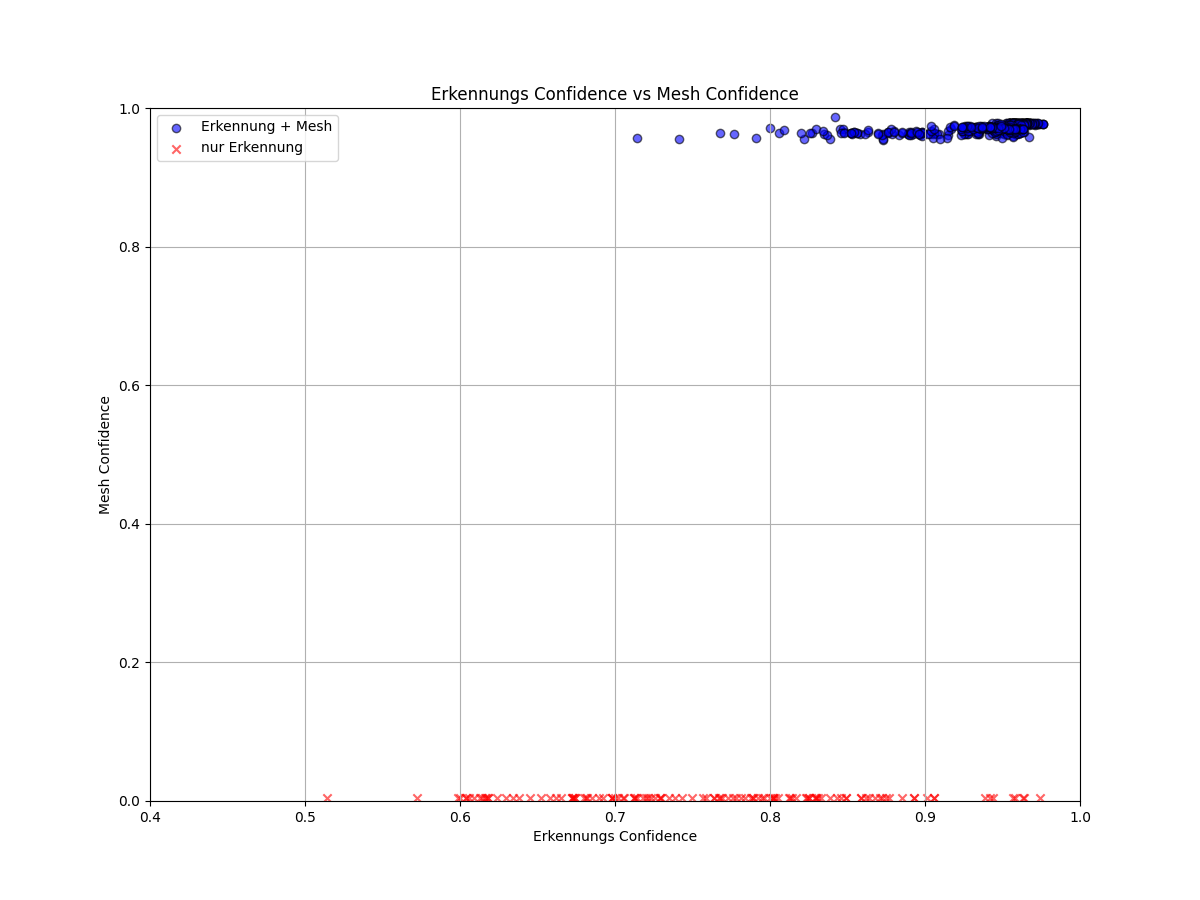
\includegraphics[width=0.55\textwidth]{data/Detection_vs_Mesh_Confidence.png}
    \caption{Confidence Score der Erkennung und FaceMesh}
    \label{fig:confidence_score_mediapipe}
\end{figure}

Obwohl beide Modelle tendenziell hohe Sicherheit in ihren Erkennungen aufweisen (> 0.95), ist die reine Gesichtserkennung deutlich robuster. Wir beobachten wiederholt Fälle, in denen das Detection-Modell hohe Confidence-Werte liefert (z.B. > 0.95), während die zugehörige FaceMesh-Erkennung entweder scheitert oder deutlich niedrigere Scores erzielt.

Die Ursache hierfür liegt in den zusätzlichen Anforderungen der FaceMesh-Erkennung. Sie ist stärker von idealen Aufnahmebedingungen abhängig. Das Gesicht muss vollständig sichtbar sein, die Perspektive geeignet, und die Bildqualität muss detaillierte Analysen erlauben. 
Störungen wie Verdeckungen oder Bewegungen beeinträchtigen die Mesh-Erkennung stärker als die reine Detektion. Zusammenfassend lässt sich festhalten, dass die Gesichtserkennung eine hohe Treffsicherheit besitzt, die Präzision der FaceMesh-Erkennung jedoch maßgeblich von der Qualität der Gesichtsinformationen im Bild beeinflusst wird.

\subparagraph{FPS / Inferenzzeit} 

Die Aufgabenstellung umfasste die Analyse und Bewertung der MediaPipe-Gesichtserkennung und -wiedererkennung hinsichtlich Inferenzgeschwindigkeit, Verarbeitungszeit und Stabilität.

Für die Gesichtserkennung wurden FPS, Verarbeitungszeit und Stabilität bei Confidence-Werten von 50\% und 80\% gemessen und verglichen. Die Gesichtserkennung erfolgte mit MediaPipe FaceMesh auf einer Webcam-Auflösung von 640×480 Pixeln über 60 Sekunden, wobei alle 5 Sekunden Messwerte erfasst wurden.

\begin{figure}
[ht]
    \centering
    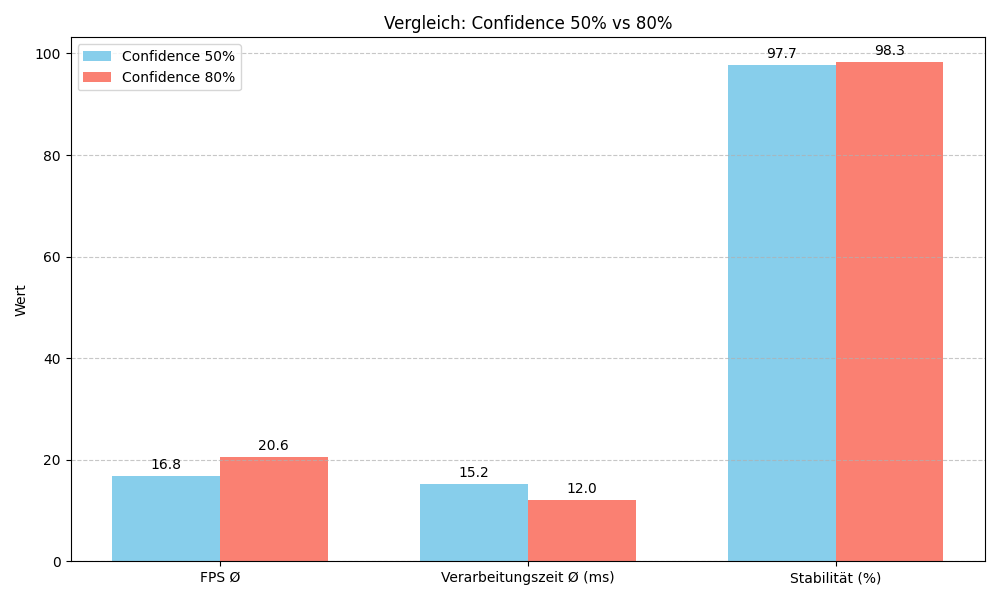
\includegraphics[width=0.55\textwidth]{data/Vergleich_Confidence_50_vs_80.png}
    \caption{Performance bei 50\% vs. 80\% Confidence}
    \label{fig:vergleich_confidence}
\end{figure}

Die Ergebnisse (siehe Abbildung \ref{fig:vergleich_confidence}) zeigen:
\begin{itemize}
    \item Die durchschnittliche Bildrate (FPS) steigt bei einem zunehmenden Confidence-Wert von 50\% auf 80\% von 16,83 FPS auf 219,48 FPS.
    \item Die durchschnittliche Verarbeitungszeit pro Frame sinkt bei einer Erhöhung des Confidence-Werts von 50\% auf 80\% von 15,18 ms auf 12,02 ms.
    \item Die Stabilität der Erkennung steigt leicht an, von 98,64\% bei 50\% auf 99,23\% bei 80\% Confidence.
\end{itemize}
Somit kann man festhalten, dass die Erhöhung des Confidence-Werts von 50\% auf 80\% zu einer signifikanten Verbesserung der Inferenzgeschwindigkeit führt. Ursache dafür ist, dass bei höherer Confidence weniger unsichere Erkennungen verarbeitet werden müssen.

Der FPS-Verlauf über die Zeit (Abbildung \ref{fig:fps_ueber_zeit}) bestätigt diese Tendenz, zeigt aber auch natürliche Schwankungen aufgrund variierender Bildinhalte (z.B. Bewegungen oder Mimik).

Zusammengefasst führt ein höherer Confidence-Wert zu einer schnelleren und stabileren Erkennung, birgt jedoch das Risiko, dass echte Gesichter unter schwierigen Bedingungen übersehen werden. Die Wahl des optimalen Confidence-Werts stellt somit einen Kompromiss zwischen Geschwindigkeit und Erkennungsempfindlichkeit dar.

\begin{figure}[ht]
    \centering
    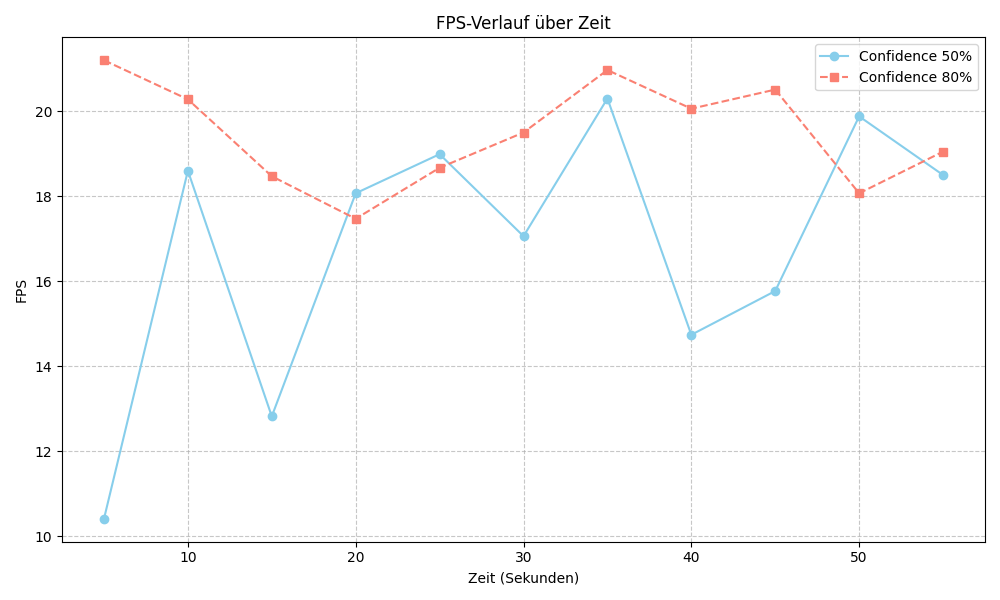
\includegraphics[width=0.55\textwidth]{data/FPS_ueber_Zeit.png}
    \caption{FPS-Werte über Zeitspanne von 60 Sekunden.}
    \label{fig:fps_ueber_zeit}
\end{figure}

Im Anschluss an die Analyse der reinen Gesichtserkennung mit MediaPipe FaceMesh wurde die Performance des erweiterten Systems zur Wiedererkennung gemessen und ausgewertet.

Die Ergebnisse sind in Abbildung \ref{fig:fps_recognition_mediapipe} dargestellt.

Die wichtigsten Ergebnisse sind:
\begin{itemize}
    \item Die durchschnittliche Bildrate (FPS) lag bei 23,55 FPS, womit eine flüssige Echtzeiterkennung gewährleistet ist.
    \item Die Verarbeitungszeit pro Frame betrug im Schnitt 22,71 ms, was eine solide Reaktionsgeschwindigkeit ermöglicht.
    \item Die Stabilität lag im Mittel bei 98,64\%, was auf eine gleichmäßige und zuverlässige Verarbeitung hinweist.
\end{itemize}

\begin{figure}[ht]
    \centering
    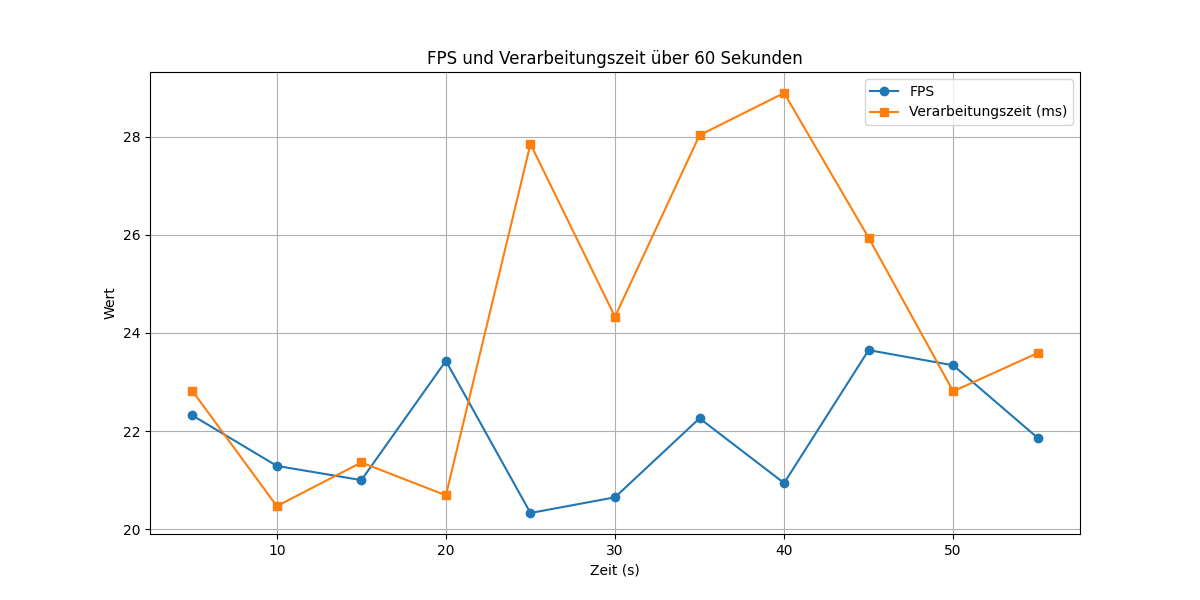
\includegraphics[width=0.55\textwidth]{data/FPS_and_Processing_Time.png}
    \caption{FPS und Verarbeitungszeit bei Wiedererkennung.}
    \label{fig:fps_recognition_mediapipe}
\end{figure}

Verglichen mit der reinen Gesichtserkennung zeigt sich, dass die Integration der Wiedererkennungslogik (Vergleich von Landmark-Distanzen) zwar die durchschnittliche Verarbeitungsgeschwindigkeit leicht reduziert, jedoch weiterhin ausreichend Echtzeitfähigkeit und hohe Stabilität gewährleistet. 
Während bei der reinen Erkennung eine Erhöhung des Confidence-Werts zu einer Steigerung der Geschwindigkeit führte, hängt die Performance der Wiedererkennung primär von der Effizienz der Landmarkverarbeitung und der Distanzberechnung ab.

Unser Programm zeigt eine für viele praktische Anwendungen ausreichende Performance. Die Gesichtserkennung und -wiedererkennung mit MediaPipe FaceMesh kann bei moderater Rechenlast stabil und in Echtzeit arbeiten. 


\paragraph{Anwendungsbeispiel: Zutrittskontrollen}

Mediapipe bietet zwar grundlegende Funktionen zur Gesichtserkennung, weist jedoch erhebliche Einschränkungen bei der zuverlässigen Wiedererkennung von Personen auf. 
Während unser System Gesichter erkennen und deren Merkmale (Landmarks) identifizieren kann, ist es primär für die Erkennung der Gesichtsstruktur konzipiert und nicht für die biometrische Identifikation.

Ein wesentliches Problem ist die langsame Anpassungsfähigkeit. Bei schnellen Bewegungen kann unser System die Wiedererkennung verlieren, wodurch Nutzer gezwungen sind, eine Position zu finden, in der sie erneut erkannt werden. 
Die verwendete Landmark-Distanz-Methode erweist sich als besonders empfindlich: Veränderungen im Gesichtsausdruck, bei Lichtverhältnissen oder der Perspektive können die Lage der Gesichtspunkte signifikant beeinflussen und damit die Wiedererkennung erschweren.

Zudem fehlen wichtige Sicherheitsfunktionen. Es gibt keinen Schutz gegen einfache Täuschungsversuche, beispielsweise könnte jemand ein Foto hochhalten und das System würde dies als echtes Gesicht erkennen. 
Dies macht die Technologie deutlich weniger robust als moderne Face-Recognition-Methoden. Auch die Verwaltung mehrerer Nutzerprofile würde bei diesem einfachen Ansatz schnell komplex und fehleranfällig werden.

Mediapipe wurde eigentlich für andere Anwendungsbereiche entwickelt, insbesondere für Augmented Reality-Anwendungen, bei denen es darum geht, virtuelle Elemente auf Gesichter zu projizieren. 
Seine Stärke liegt in der präzisen Erkennung von Gesichtspunkten, nicht in der Identifikation bestimmter Personen.

Für eine zuverlässige Zutrittskontrolle wären zusätzliche Komponenten erforderlich:
\begin{itemize}
    \item Ein Vergleichssystem mit Face Embeddings und Klassifikationsalgorithmen
    \item Lebenderkennung, um Angriffe mit Fotos oder Videos zu verhindern
    \item Ein zuverlässiges Management-System für gespeicherte Nutzerprofile
\end{itemize}

Zusammenfassend kann Mediapipe durchaus als Baustein für einfache Zugangskontrollen in nicht-kritischen Bereichen dienen (etwa für private Projekte), ist jedoch für sicherheitsrelevante Anwendungen ohne erhebliche Erweiterungen und Kombinationen mit anderen Technologien nicht geeignet. 
Die Stärken des Systems liegen eindeutig in der grundlegenden Gesichtserkennung, während für die zuverlässige Wiedererkennung und Identifikation von Personen fortgeschrittenere Lösungen notwendig sind.

\subsubsection{Vergleich von YOLO und MediaPipe}
\paragraph{Confidence Score}
\paragraph{FPS / Inference Time}

\subsubsection{Manipulierte Gesichtserkennung}
\paragraph{Angriffsmethoden auf Gesichtserkennungssysteme}
\paragraph{Testen der Robustheit gegen Manipulationen}
\paragraph{Möglichkeiten zur Absicherung}

\subsubsection{Projektdokumentation}
\paragraph{Vorgehensmodell und Teamorganisation}
\paragraph{Dokumentation des Projektmanagements}